%compile with pdflatex on papeeria

\documentclass[a4paper,12pt]{article}


\usepackage{fontawesome}
\usepackage{fancyhdr}
\usepackage{fancyheadings}
\usepackage[ngerman,german]{babel}
\usepackage{german}
\usepackage[utf8]{inputenc}
%\usepackage[latin1]{inputenc}
\usepackage[active]{srcltx}
%\usepackage{svg}
%\usepackage{algorithm}
%\usepackage[noend]{algorithmic}
\usepackage{eurosym}
\usepackage{amsmath}
\usepackage{amssymb}
\usepackage{amsthm}
\usepackage{bbm}
\usepackage{enumerate}
\usepackage{graphicx}
\usepackage{ifthen}
\usepackage{listings}
\usepackage{enumitem}
%\usepackage{struktex}
\usepackage{hyperref}
\usepackage{tikz}
\usepackage{float}
\usepackage{subcaption}
\usepackage{array}
\captionsetup{compatibility=false}
\captionsetup[subfigure]{labelformat=empty}

\usepackage{pgfplots}
\pgfplotsset{compat=1.15}
\usepackage{mathrsfs}
\usetikzlibrary{arrows}

\definecolor{ccqqqq}{rgb}{0.8,0,0}
\definecolor{kolorwykresu}{rgb}{0.07,0.04,0.56}

\pagenumbering{gobble}

\usepackage{tabularray}
\usepackage{multirow}
\usepackage{booktabs,tabularx}

%\DeclareMathSymbol{\shortminus}{\mathbin}{AMSa}{"39}

\renewcommand\tabularxcolumn[1]{m{#1}}% for vertical centering text in X column

\newcolumntype{L}[1]{>{\raggedright\let\newline\\\arraybackslash\hspace{0pt}}m{#1}}
\newcolumntype{C}[1]{>{\centering\let\newline\\\arraybackslash\hspace{0pt}}m{#1}}
\newcolumntype{R}[1]{>{\raggedleft\let\newline\\\arraybackslash\hspace{0pt}}m{#1}}

\newcolumntype{Y}{>{\centering\arraybackslash}X}

%%%%%%%%%%%%%%%%%%%%%%%%%%%%%%%%%%%%%%%%%%%%%%%%%%%%%%
%%%%%%%%%%%%%% EDIT THIS PART %%%%%%%%%%%%%%%%%%%%%%%%
%%%%%%%%%%%%%%%%%%%%%%%%%%%%%%%%%%%%%%%%%%%%%%%%%%%%%%
\newcommand{\Fach}{1. Klausur aus der Mathematik}
\newcommand{\Name}{}
\newcommand{\datum}{}
\newcommand{\Matrikelnummer}{}
\newcommand{\Semester}{Q12}
\newcommand{\Uebungsblatt}{} %  <-- UPDATE ME
%%%%%%%%%%%%%%%%%%%%%%%%%%%%%%%%%%%%%%%%%%%%%%%%%%%%%%
%%%%%%%%%%%%%%%%%%%%%%%%%%%%%%%%%%%%%%%%%%%%%%%%%%%%%%

\setlength{\parindent}{0em}
\topmargin -1.0cm
\oddsidemargin 0cm
\evensidemargin 0cm
\setlength{\textheight}{9.2in}
\setlength{\textwidth}{6.0in}

%%%%%%%%%%%%%%%
%% Aufgaben-COMMAND
\newcommand{\Aufgabe}[1]{
  {
  \vspace*{0.5cm}
  \textsf{\textbf{Aufgabe #1}}
  \vspace*{0.2cm}
  
  }
}
%%%%%%%%%%%%%%
\hypersetup{
    pdftitle={\Fach{}: Übungsblatt \Uebungsblatt{}},
    pdfauthor={\Name},
    pdfborder={0 0 0}
}

\lstset{ %
language=java,
basicstyle=\footnotesize\tt,
showtabs=false,
tabsize=2,
captionpos=b,
breaklines=true,
extendedchars=true,
showstringspaces=false,
flexiblecolumns=true,
}

\newcommand*{\quadratbox}{\textbf{\fbox{\phantom{\huge{?}}}}}%

\title{Übungsblatt \Uebungsblatt{}}
\author{\Name{}}

\begin{document}

\fancyhead{}
\fancyhead[C]{\includegraphics[height=2.5cm]{lukasLogoV2.png}
\vspace{2cm}
}

\thispagestyle{fancy}

\lhead{
%\vspace{1cm}
  \sf \LARGE \Fach{} %\small \Name{} - \Matrikelnummer{}
}
\rhead{\sf \Semester{}   \datum{}}


\vspace*{0.2cm}

\vspace{4cm}
Alle Lösungen müssen mit Nebenrechnungen und Begründungen nachvollziehbar sein!

%\rhead{\sf \Semester{} }
\vspace*{0.2cm}

%\begin{center}
%%\LARGE \sf \textbf{Übungsblatt \Uebungsblatt{}}
%\end{center}
%\vspace*{0.2cm}

%%%%%%%%%%%%%%%%%%%%%%%%%%%%%%%%%%%%%%%%%%%%%%%%%%%%%%
%% Insert your solutions here %%%%%%%%%%%%%%%%%%%%%%%%
%%%%%%%%%%%%%%%%%%%%%%%%%%%%%%%%%%%%%%%%%%%%%%%%%%%%%%

\vspace{1cm}
  Name: \underline{\hspace{7cm}}
  \hfill
  Datum: \underline{\hspace{4cm}}

\vspace{0.8cm}

%\textbf{Hinweise:} Der Lösungsweg muss nachvollziehbar sein. Arbeitszeit \textbf{45 Minuten}.
%\vspace{0,5cm}Die Rechenwege müssen nachvollziehbar sein!
%
%\vspace{0,5cm} {TEIL A} - ohne Hilfsmittel - Bearbeitungszeit 30 Minuten
%\vspace {0.8cm}
% 
%GEOMETRIE


\begin{center}
  \begin{tblr}{
      width=1\linewidth,
      colspec = {Q[c,5em]Q[c,2em]Q[c,2em]Q[c,2em]Q[c,2em]Q[c,2em]Q[c,2em]Q[c,2em]Q[c,2em]Q[c,2em]Q[c,2em]Q[c,5em]Q[c,3em]},
      rowspec = {Q[m]Q[m]Q[m]Q[m]Q[m]Q[m]Q[m]Q[m]Q[m]Q[m]Q[m]Q[m]Q[m]},
      colsep = 0mm,
      %row{1} = {2em,azure2,fg=white,font=\large\bfseries\sffamily},
      row{1} = {2em,font=\large\bfseries\sffamily},
      hlines, vlines,
    }
    \textbf{Aufgabe} & \textbf{1} & \textbf{2} & \textbf{3} & 
    \textbf{4} & \textbf{5} & \textbf{6}& \textbf{7}& \textbf{8}& \textbf{9}& \textbf{10}&
    \textbf{Gesamt} & \textbf{Note}\\
    {Mögliche \\ Punkte} & 4 & 4 & 4 & 8 & 13 & 13 & 3 & 6 & 7 & 3 & 65 \\
    {Erreichte \\ Punkte} &  &  &  &  & & & & & & & & \\
  \end{tblr}
\end{center}

\vspace{0.3cm}
%\newpage\null\thispagestyle{empty}\newpage
\newpage
\vspace{1,5cm} {TEIL A} - ohne Hilfsmittel. Bearbeitungszeit 25 min.
\vspace {0,2cm}

\Aufgabe{1: (2,5BE+1,5BE)}

Geben Sie eine Integralfreie Darstellung an und interpretieren Sie geometrisch das Ergebnis bei $e$.
\begin{enumerate}[label={\alph*)}]
  \item $\int \frac{1-2x}{x^2}\, dx$
  \item $\int 4xe^{-x^2}\, dx$
\end{enumerate}

\Aufgabe{2: (2BE+2BE)}
Gegeben ist die Funktion $f$ mit untenstehendem Graphen $G_f$.
\begin{enumerate}[label={\alph*)}]
  \item Tino hat das Integral $\int_{-2}^{0} f(x)\, dx$ berechnet, dabei erhielt er den Wert -3. Nehmen Sie die Stellung zu seinem Ergebnis.
  \begin{figure}[H]
    \vspace{0cm}
    \centering
    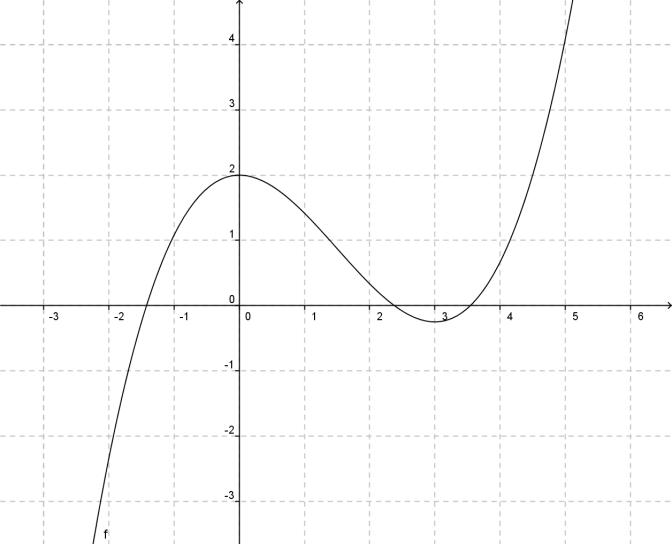
\includegraphics[width=0.5\linewidth]{Q12_SA_240103_1.jpg}
  \end{figure}

\item Betrachten Sie nun die Integralfuntion $\int_1^{x} f(t)\, dt$. Begründen Sie, warum weder der Graph $G_1$ noch der Graph $G_2$ ein Graph dieser Funktion sein kann.

\begin{minipage}[t]{0.5\textwidth}
  \begin{figure}[H]
    \vspace{0cm}
    \centering
    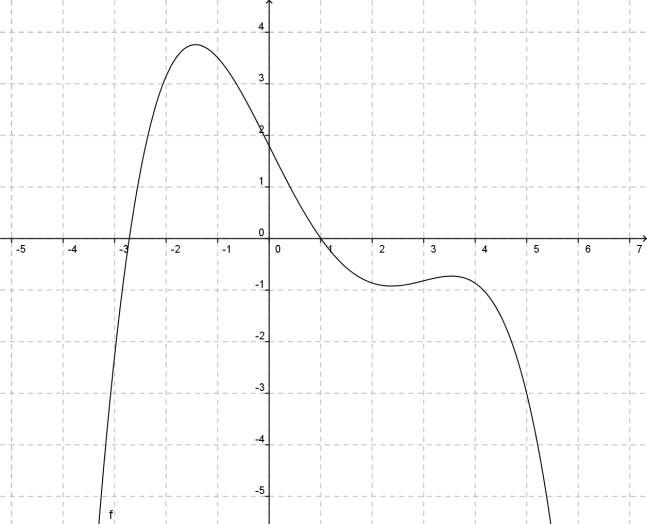
\includegraphics[width=0.8\linewidth]{Q12_SA_240103_2.jpg}
  \end{figure}
\captionof*{figure}{Graph $G_1$}
\end{minipage}
%\hspace*{0.75cm}
\begin{minipage}[t]{0.5\textwidth}
  \begin{figure}[H]
    \vspace{0cm}
    \centering
    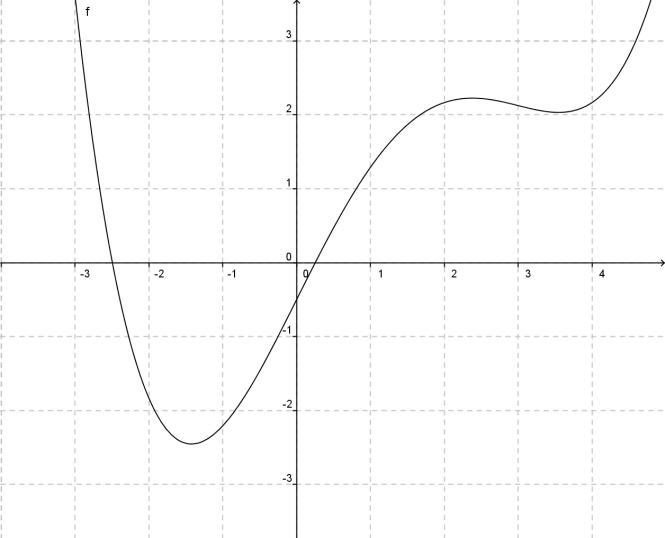
\includegraphics[width=0.8\linewidth]{Q12_SA_240103_3.jpg}
  \end{figure}
\captionof*{figure}{Graph $G_2$}
\end{minipage}


\end{enumerate}


\Aufgabe{3: (4BE)}
Die Abbildung zeigt den Graphen $G_g$ einer in $\mathbb{IR}$ definierten, differenzierbaren Funktion $g$.

  \begin{figure}[H]
    \vspace{0cm}
    \centering
    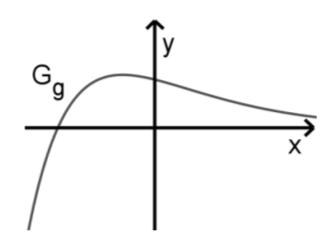
\includegraphics[width=0.3\linewidth]{Q12_SA_240103_4.jpg}
  \end{figure}

Betrachtet wird eine in $\mathbb{IR}$ definierte Funktion $f$, für deren erste Ableitungsfunktion $f'(x) = e^{g(x)}$ gilt.
Untersuchen Sie, ob der Graph von $f$ einen Wendepunkt hat.


\vspace{1cm}
STOCHASTIK



\Aufgabe{4: (2BE+3BE+2BE+1BE)}
Ein Glücksrad hat einen schwarzen, einen roten und einen goldenen Sektor. Beim Drehen tritt schwarz mit $5p$ ein und rot mit $4p$.
\begin{enumerate}[label={\alph*)}]
  \item Geben Sie die Werte an, die $p$ bei diesem Glücksrad annehmen kann.\\

  Der Wert für $p$ sei nun 0,1. \\
  Es wird einmal gedreht und als Spiel wurde vereinbart: der Einsatz beträgt 2\euro. Bleibt der Zeiger auf ‚Gold‘ werden 10\euro ausgezahlt, bei ‚Rot‘ beträgt die Auszahlung 1\euro und bei ‚Schwarz‘ erhält man keine Auszahlung.
\item Bestimmen Sie die Wahrscheinlichkeitsverteilung der Zufallsgröße $X:$ ,,Gewinn des Spielers pro Spiel''.
\item Würden Sie sich bei diesem Spiel beteiligen? Begründen Sie Ihre Antwort.
\item Ändern Sie den Einsatz so ab, dass das Spiel fair ist.
\end{enumerate}


\newpage
\vspace{1,5cm} {TEIL B} - mit Hilfsmitteln. Bearbeitungszeit 65 min.
\vspace {0,2cm}

ANALYSIS

\Aufgabe{5: (7BE+2BE+4BE)}
Gegeben ist die Funktion $f: x \rightarrow \frac{1}{2} x \cdot e^{-0,1x+2}$ mit ihrem Graphen $G_f$ (s. unten).\\
Die Funktion $F: x \rightarrow (5x-50) \cdot e^{-0,1x+2}$ ist eine Stammfunktion von $f$.
  \begin{figure}[H]
    \vspace{0cm}
    \centering
    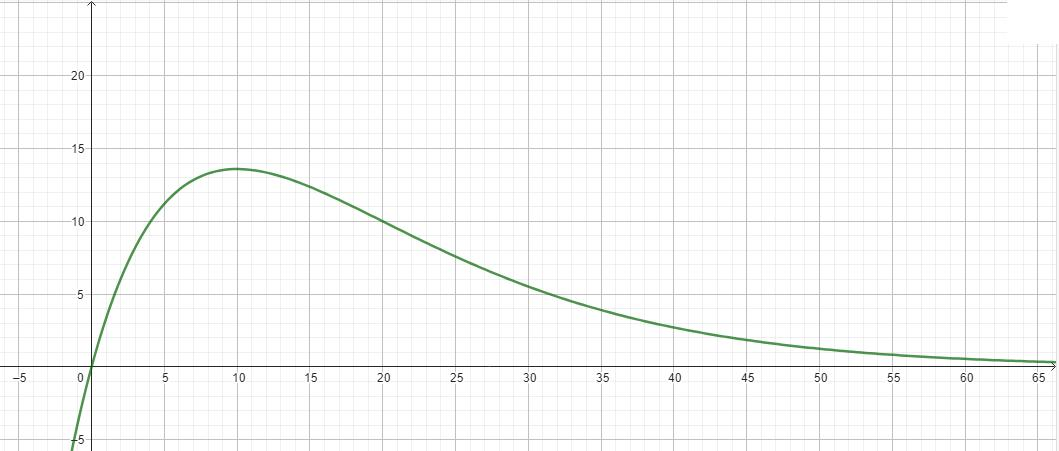
\includegraphics[width=0.8\linewidth]{Q12_SA_240103_5.jpg}
  \end{figure}

\begin{enumerate}[label={\alph*)}]
  \item Bestimmen Sie das Krümmungsverhalten der Funktion $f$ sowie die Lage des Wendepunkts.
  \item Bestimmen Sie die Gleichung der Wendetangente.
%\textcolor{red}{
  \item Berechnen Sie anhand der Abbildung näherungsweise $\int_5^{30} f(x)\, dx$ und bestimmen Sie die prozentuale Abweichung dieses Wertes zum tatsächlichen Wert des Integrals.
%  }
\end{enumerate}

\Aufgabe{6: (1,5BE+3,5BE+3BE+2BE+3BE)}
Gegeben ist die Funktion $f: x \rightarrow \frac{4}{x+2}$ mit ihrem Definitionsbereich $D_f$, sowie die Gerade $g$ mit der Gleichung: $g(x) = -2x+4$.

\begin{enumerate}[label={\alph*)}]
  \item Zeichnen Sie den Graphen von $f$ im Bereich $[-4; 6]$
  \item Der Graph von $f$ schließt mit der $x$- Achse und den Geraden $x=-1$ und $x=a$, $a \ge -1$ eine Fläche ein. Bestimmen Sie den Wert von $a$ so, dass diese Fläche den Inhalt 8 FE hat.
  \item Für $a \rightarrow +\infty$ wird die Fläche der Aufgabe b) unbegrenzt. Untersuchen Sie den Inhalt der Fläche und interpretieren Sie das Ergebnis.
  \item Schraffieren Sie die Fläche, die durch das Integral $\int_{-1}^{4}[f(x)-g(x)] dx$ dargestellt wird und begründen Sie anhand der Zeichnung, ob das Integral einen positiven oder negativen Wert hat 

    %Für meinen Kurs statt 2c und hypergeom. Aufgabe:
%Die Punkte A(-1|4) und B(6|0, 5) liegen auf 𝐺𝑓 ; zwischen diesen beiden Punkten verläuft 𝐺𝑓 unterhalb der
%Strecke [AB].
  \item Berechnen Sie den Inhalt der Fläche, die von $G_f$ und der Strecke $[A B]$ eingeschlossen wird.
\end{enumerate}


\Aufgabe{7: (3BE)}
Gegeben sei folgende Definition eines Drehkörpervolumens:

  \begin{figure}[H]
    \vspace{0cm}
    \centering
    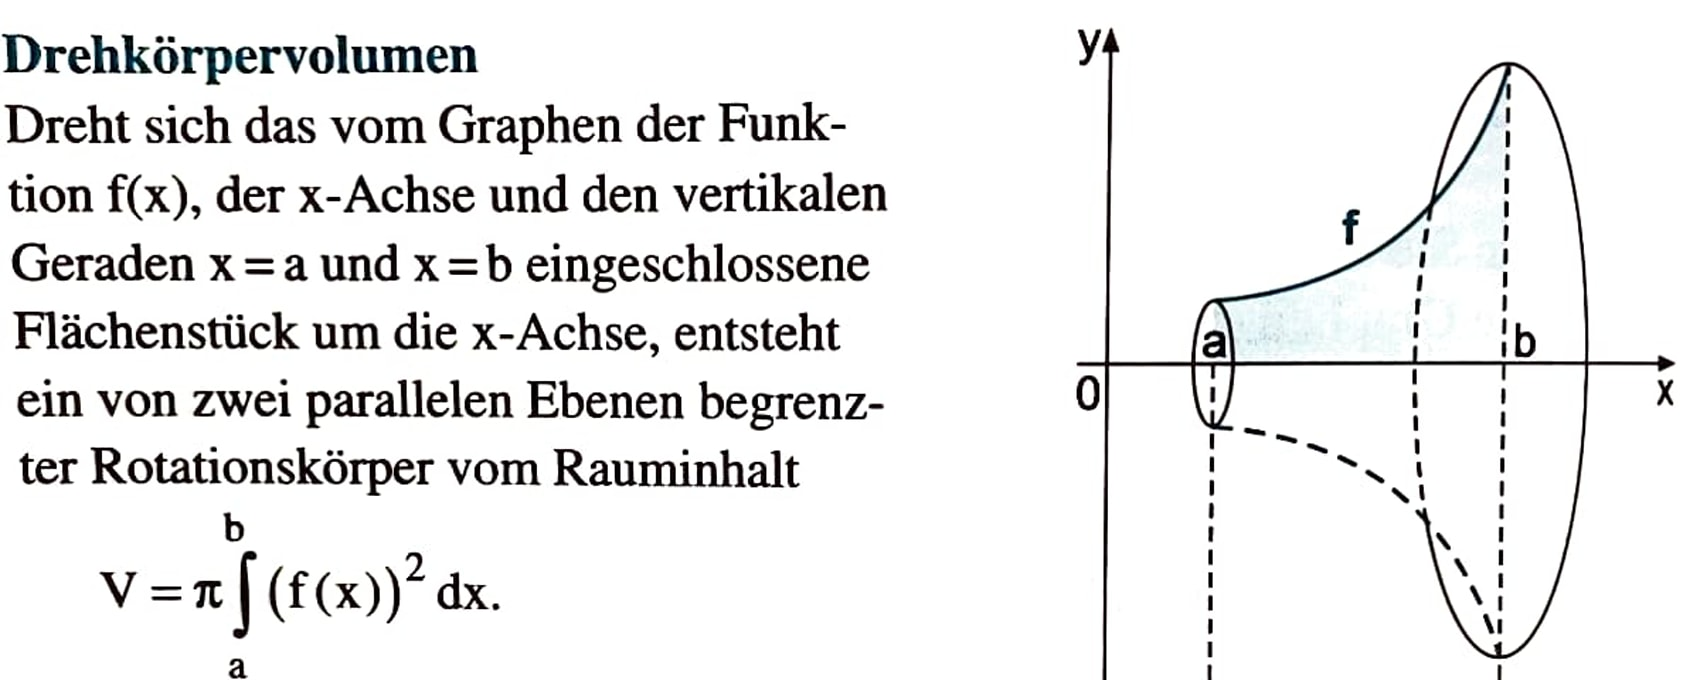
\includegraphics[width=0.7\linewidth]{Q12_SA_240103_6.jpg}
  \end{figure}

Das vom Graphen der Funktion $f: x\rightarrow \sqrt{x}, x \in [0; 4]$ und der $x$-Achse eingeschlossene Flächenstück rotiert um die $x$-Achse. Berechnen Sie das Volumen des dabei entstehenden Rotationskörpers.


\Aufgabe{8: (2BE+1BE+3BE)}
Die Abbildung zeigt den Graphen einer in $\mathbb{R}$ definierten Funktion $f: x\rightarrow f(x)$.

  \begin{figure}[H]
    \vspace{0cm}
    \centering
    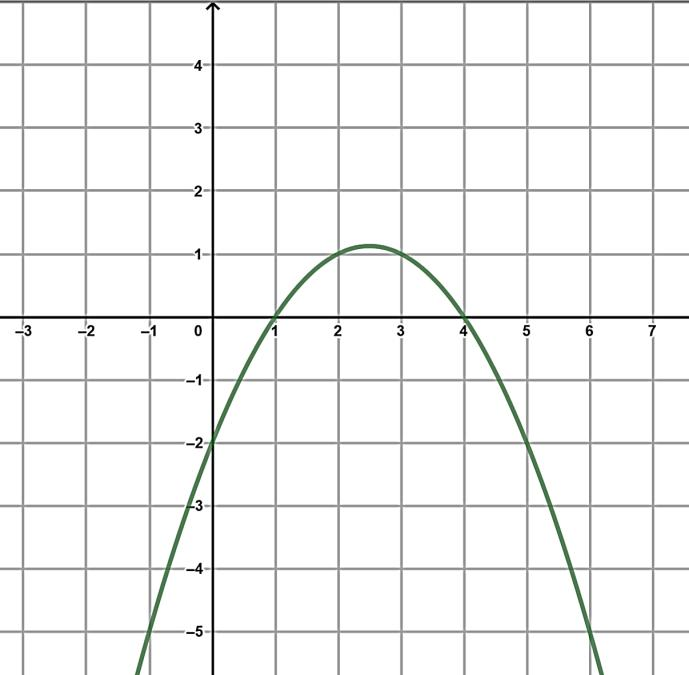
\includegraphics[width=0.7\linewidth]{Q12_SA_240103_7.jpg}
  \end{figure}

Gegeben sei weiter der Term der Integralfunktion mit $I_1 (x)= \int_1^x f(t)\, dt$
\begin{enumerate}[label={\alph*)}]
  \item Bestimmen Sie nachvollziehbar Lage und Anzahl der Nullstellen der Integralfunktion.
  \item Geben Sie das Intervall an, in dem die Integralfunktion monoton steigt.
  \item Bestimmen Sie näherungsweise die Werte $I_1 (4)$ und $I_1 (-1)$ und skizzieren Sie mit Hilfe Ihrer Ergebnisse den Graphen der Integralfunktion in die Abbildung für $-1 \le x \le 6$.
\end{enumerate}

\vspace{1cm}
STOCHASTIK

\Aufgabe{9: (2BE+3BE+2BE)}
\begin{center}
  \begin{tblr}{
      width=1\linewidth,
      colspec = {Q[c,6em]Q[c,3em]Q[c,3em]Q[c,3em]Q[c,3em]Q[c,3em]},
      rowspec = {Q[m]Q[m]Q[m]Q[m]Q[m]Q[m]},
      colsep = 0mm,
      %row{1} = {2em,azure2,fg=white,font=\large\bfseries\sffamily},
      %row{1} = {2em,font=\large\bfseries\sffamily},
      %hlines, 
      vlines,
    }
        \hline
        $x_i$ & 0 & 1 & 2 & 3 & 4 \\
        \hline
        $P(X\le x_i)$ & & & 0,65 & 0,8 & 1  \\
        \hline
  \end{tblr}
\end{center}

Bei einem Test werden vier Fragen gestellt. Die Zufallsgröße $X$ beschreibt die Anzahl der richtigen Antworten. Die Wahrscheinlichkeitsverteilung von $X$ ist symmetrisch, d.h. es gilt $P(X=0) = P(X=4)$ und $P(X=1) = P(X=3)$. Die Wahrscheinlichkeitsverteilung zeigt die Wahrscheinlichkeitswerte $P(X\le x_i)$ für $x_i \in \{2; 3; 4\}$.

\begin{enumerate}[label={\alph*)}]
  \item Tragen Sie die fehlenden Werte ein.
  \item Mit welcher Wahrscheinlichkeit werden genau drei Fragen richtig beantwortet?
  \item Bestimmen Sie $P(X>1)$.
\end{enumerate}


\Aufgabe{10: (3BE)}
Frau R. hat aus einer großen Lebkuchenpackung noch einige Lebkuchen für ihren Kollegen übriggelassen. Von den noch verbleibenden 20 Lebkuchen sind aber nur noch 5 Lebkuchen mit weißer Glasur darunter.  Der Kollege greift blind in die Verpackung und nimmt sich 4 Lebkuchen heraus. Bestimmen Sie die Wahrscheinlichkeit, dass sich darunter mindestens 3 Lebkuchen mit weißer Glasur befinden?

\vspace{2cm}
\centerline{Viel Erfolg \faThumbsOUp }

\newpage
  \begin{figure}[H]
    \vspace{0cm}
    \centering
    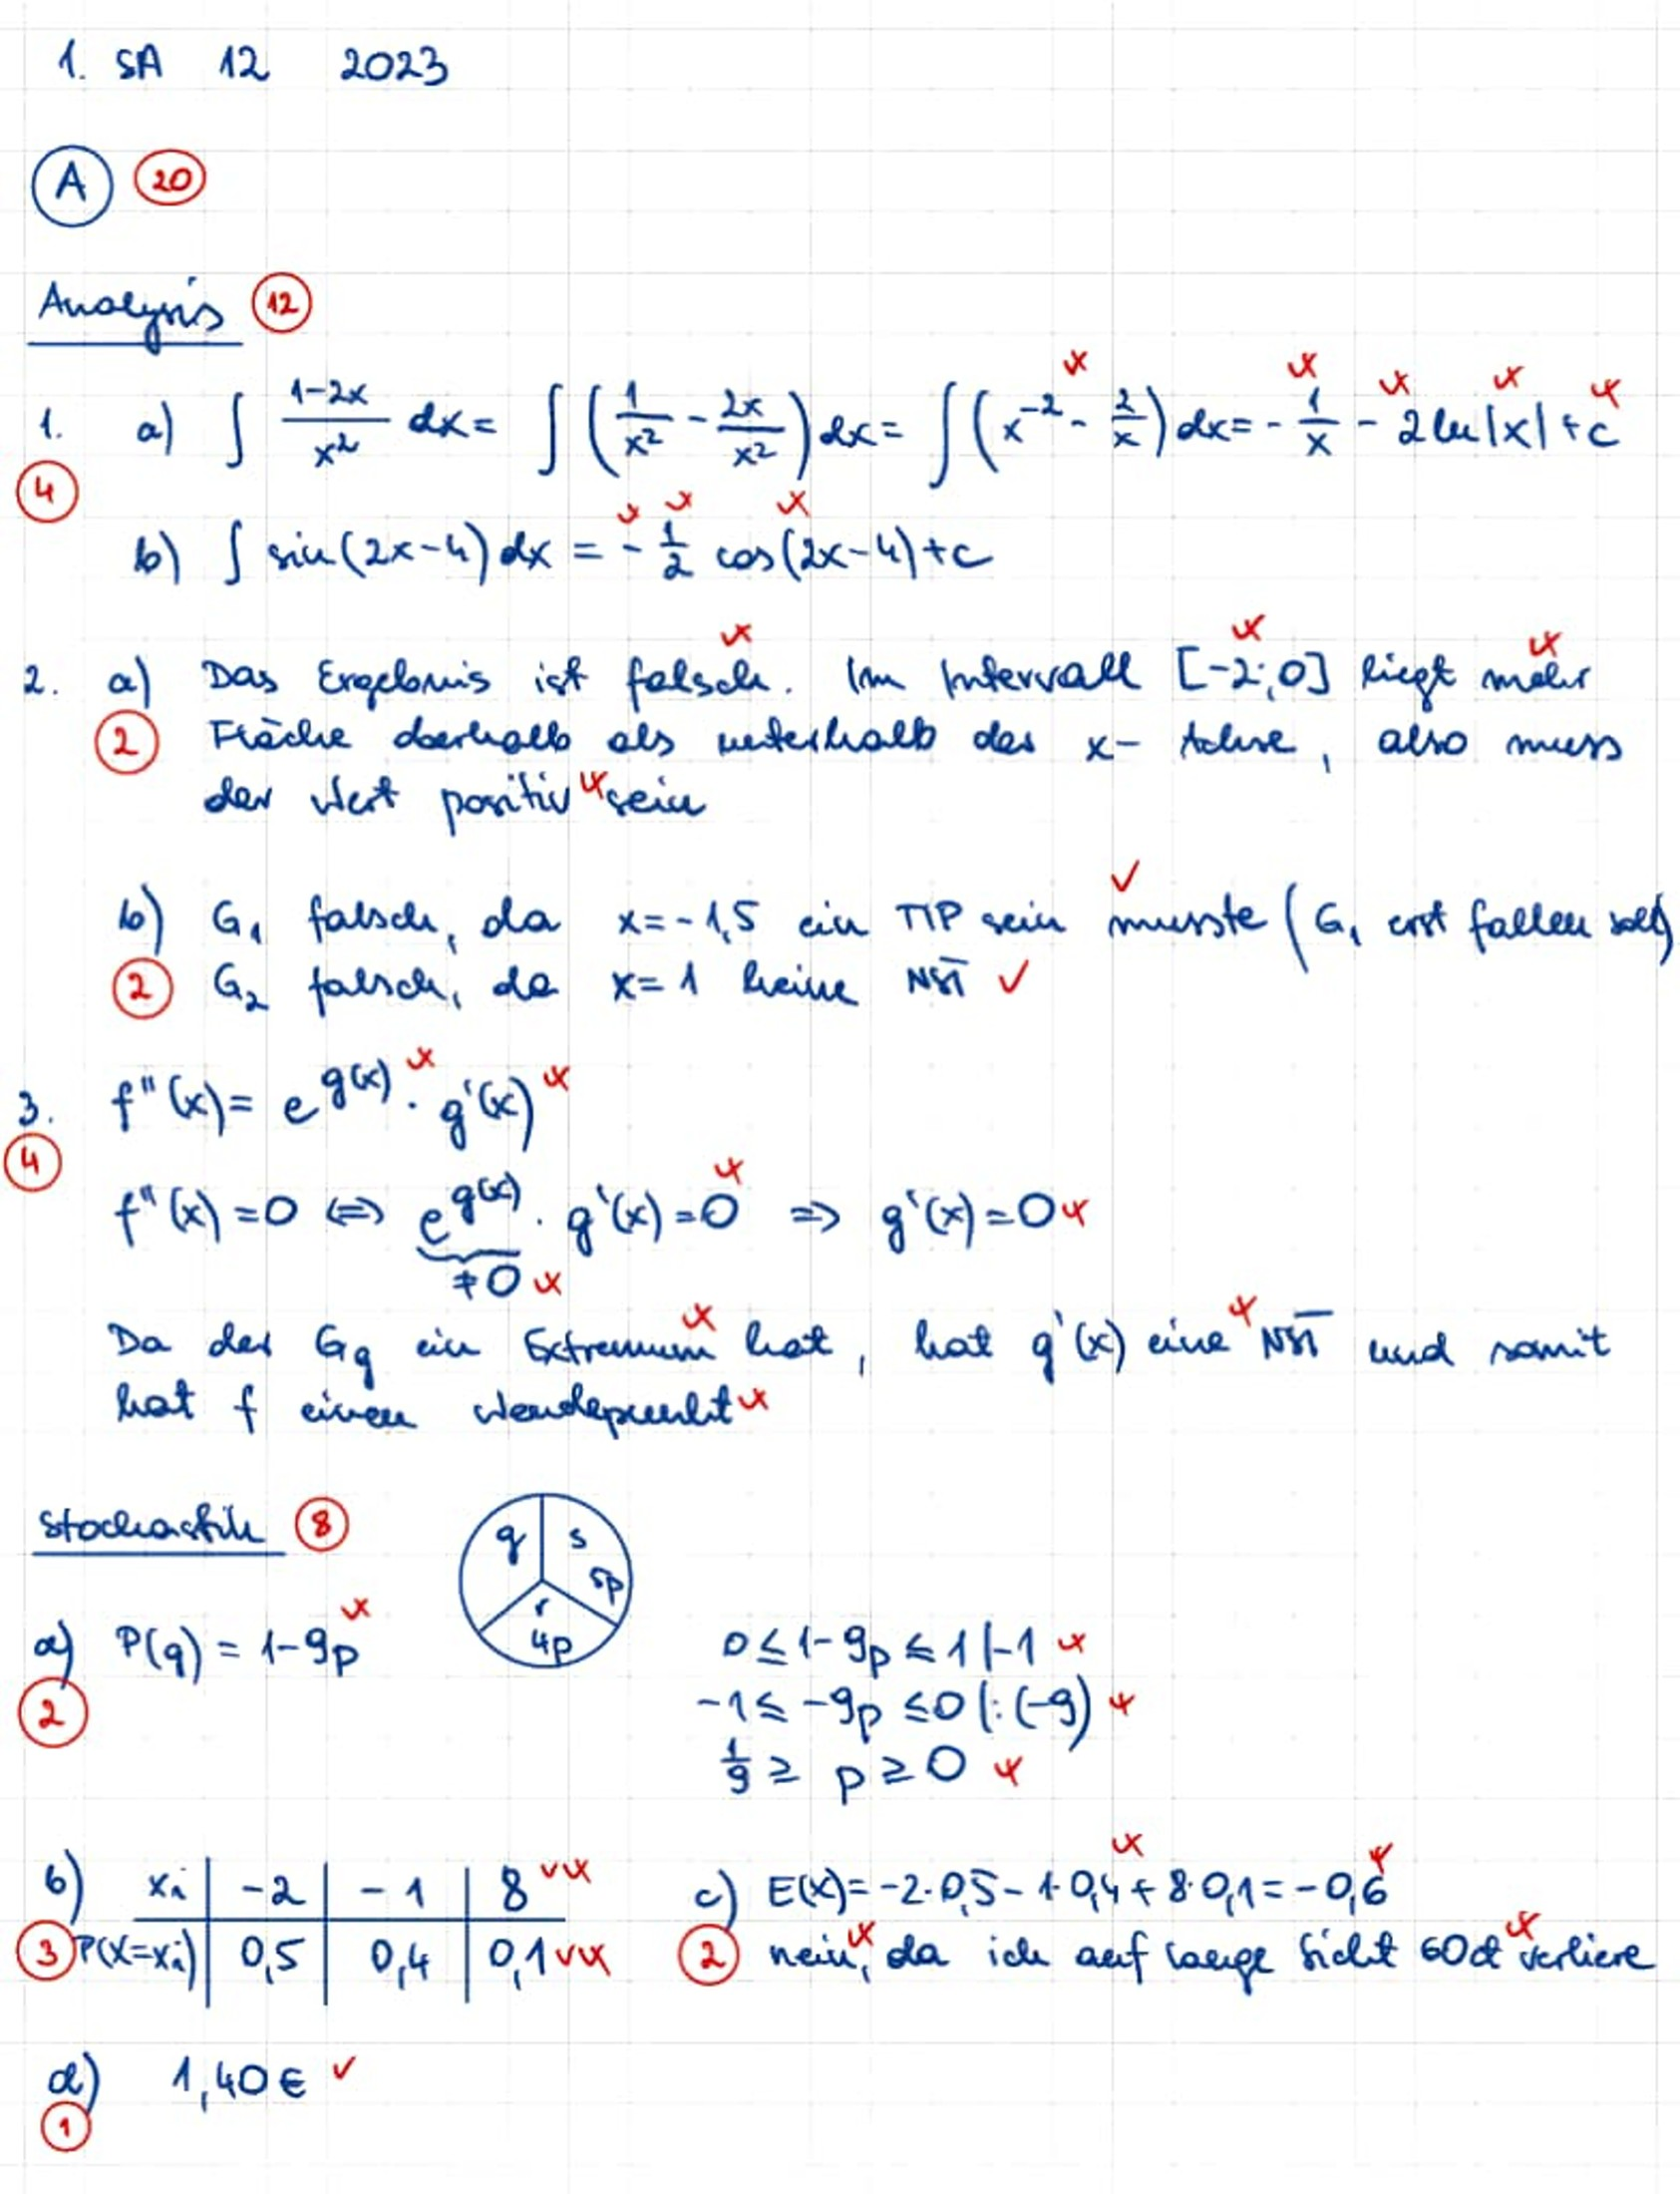
\includegraphics[width=1.2\linewidth]{Q12_SA_240103_8.jpg}
  \end{figure}

\newpage
  \begin{figure}[H]
    \vspace{0cm}
    \centering
    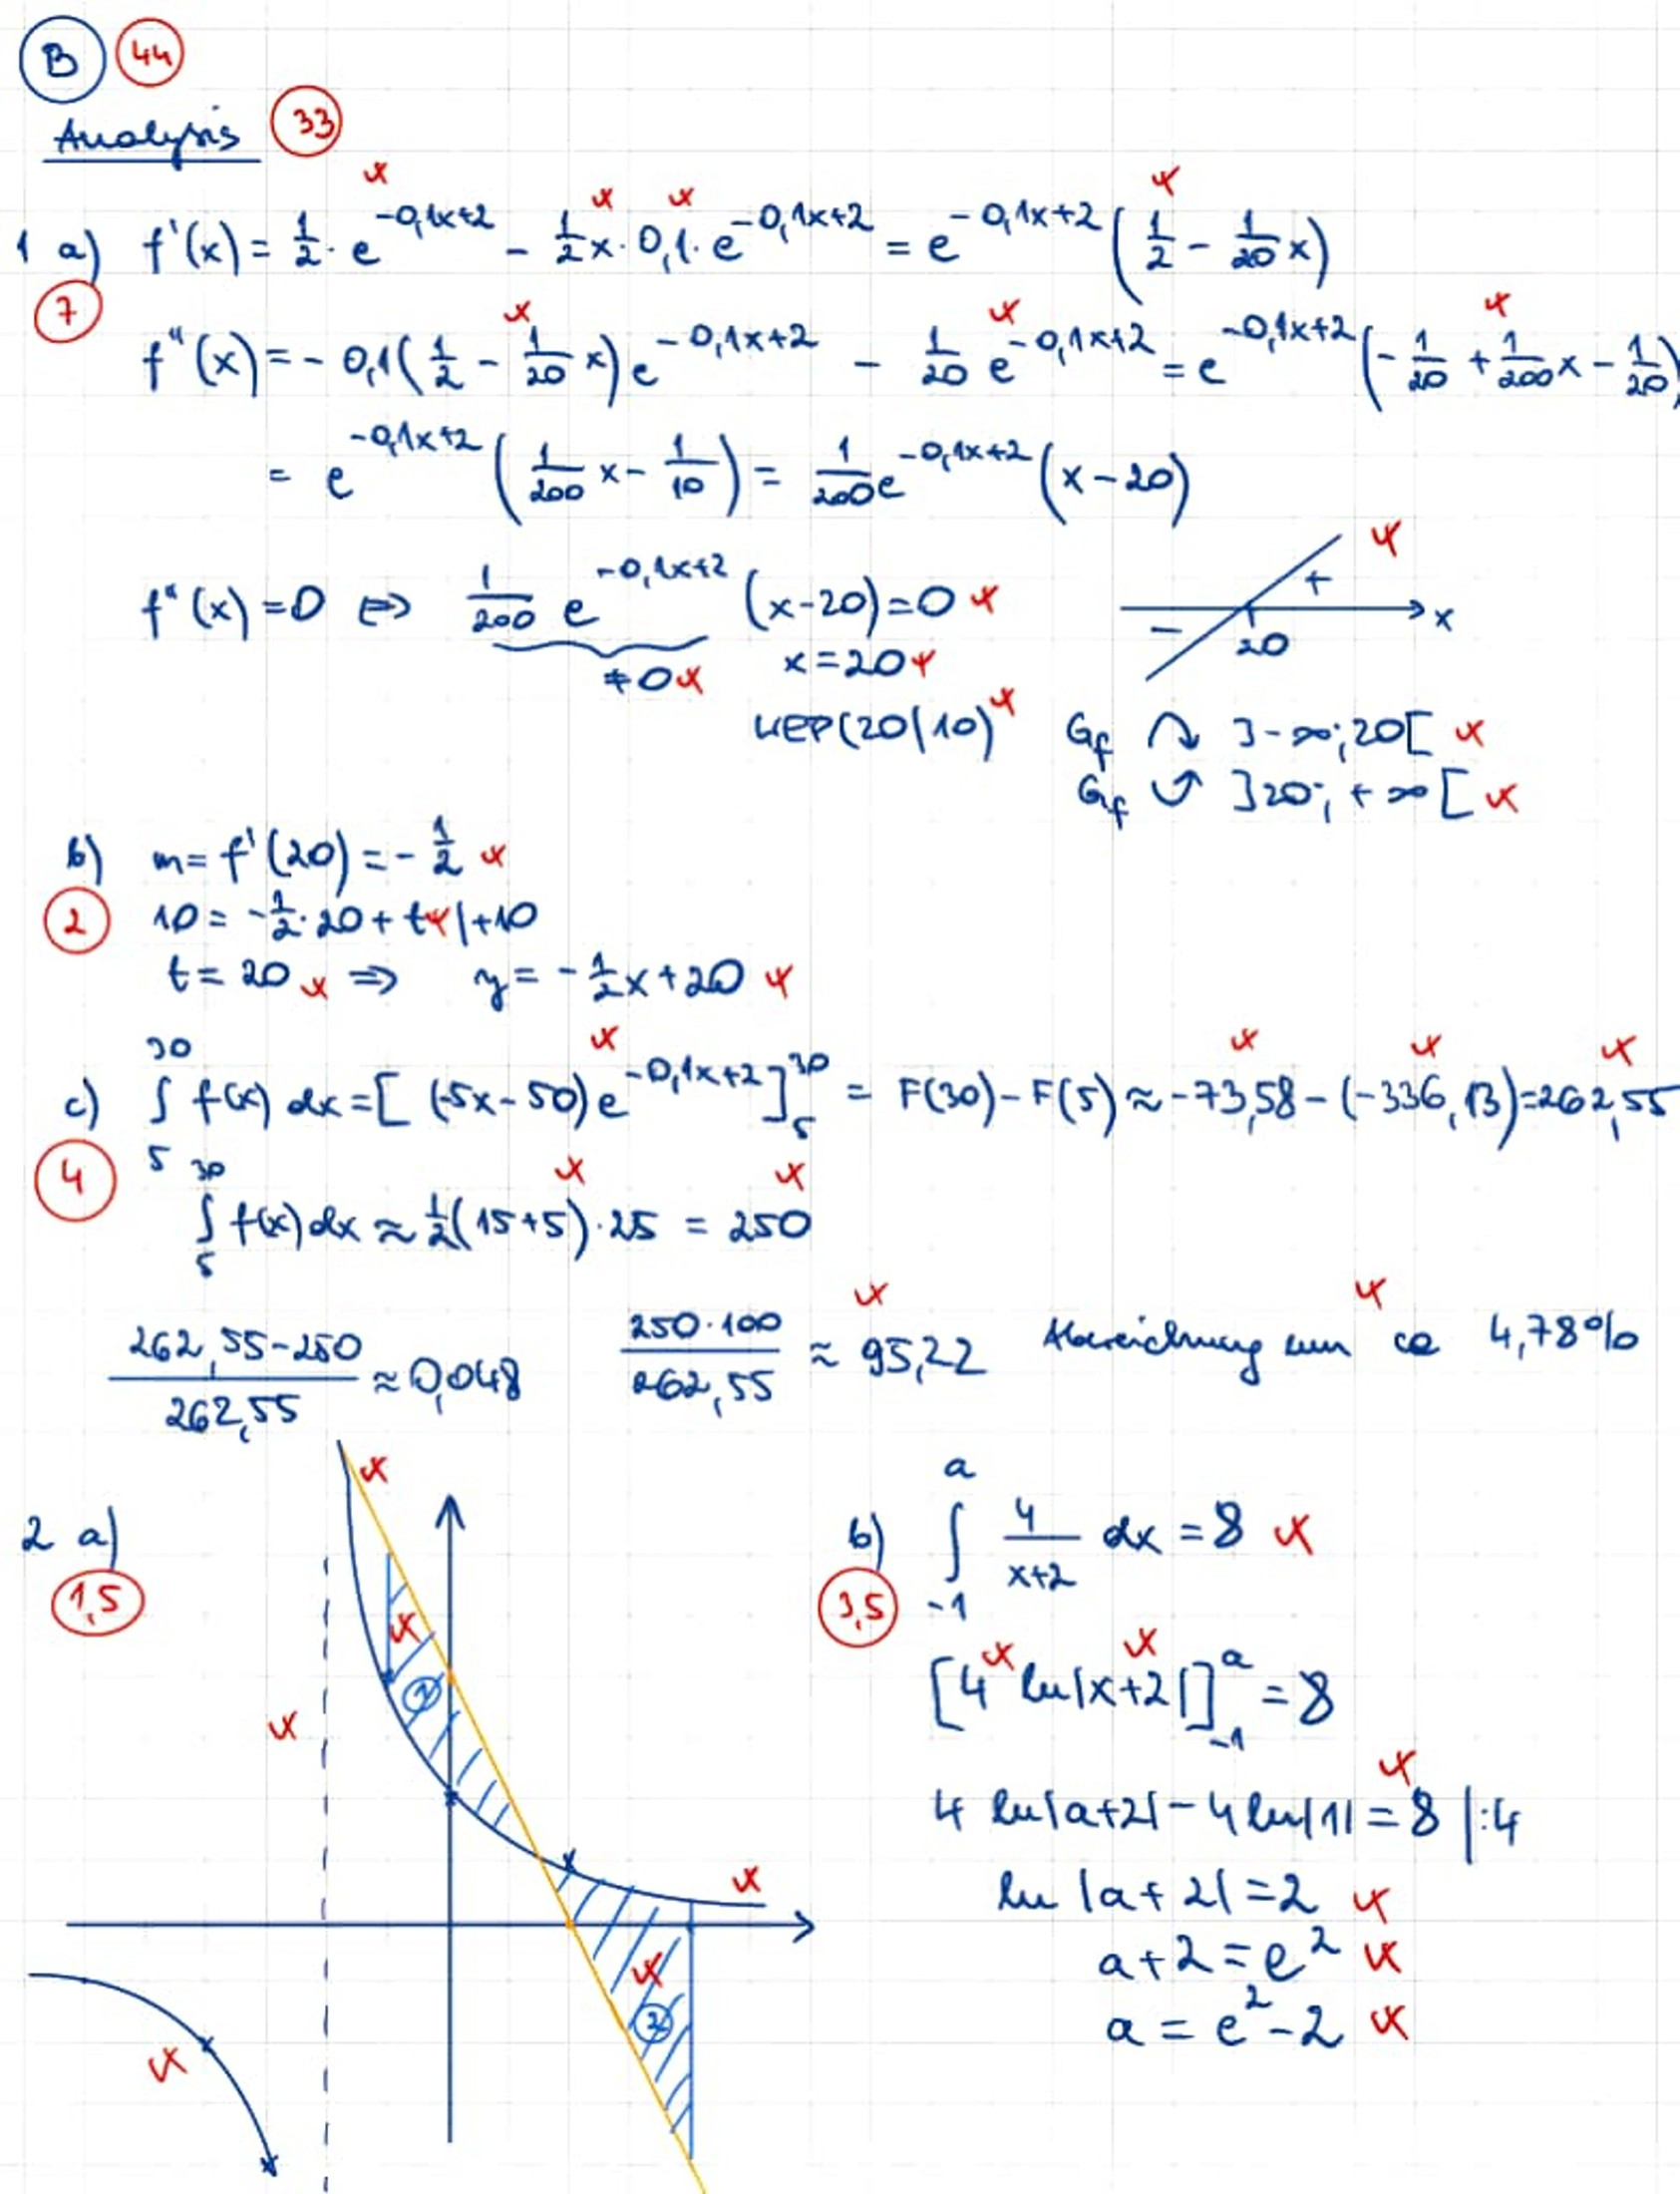
\includegraphics[width=1.2\linewidth]{Q12_SA_240103_9.jpg}
  \end{figure}

\newpage
  \begin{figure}[H]
    \vspace{0cm}
    \centering
    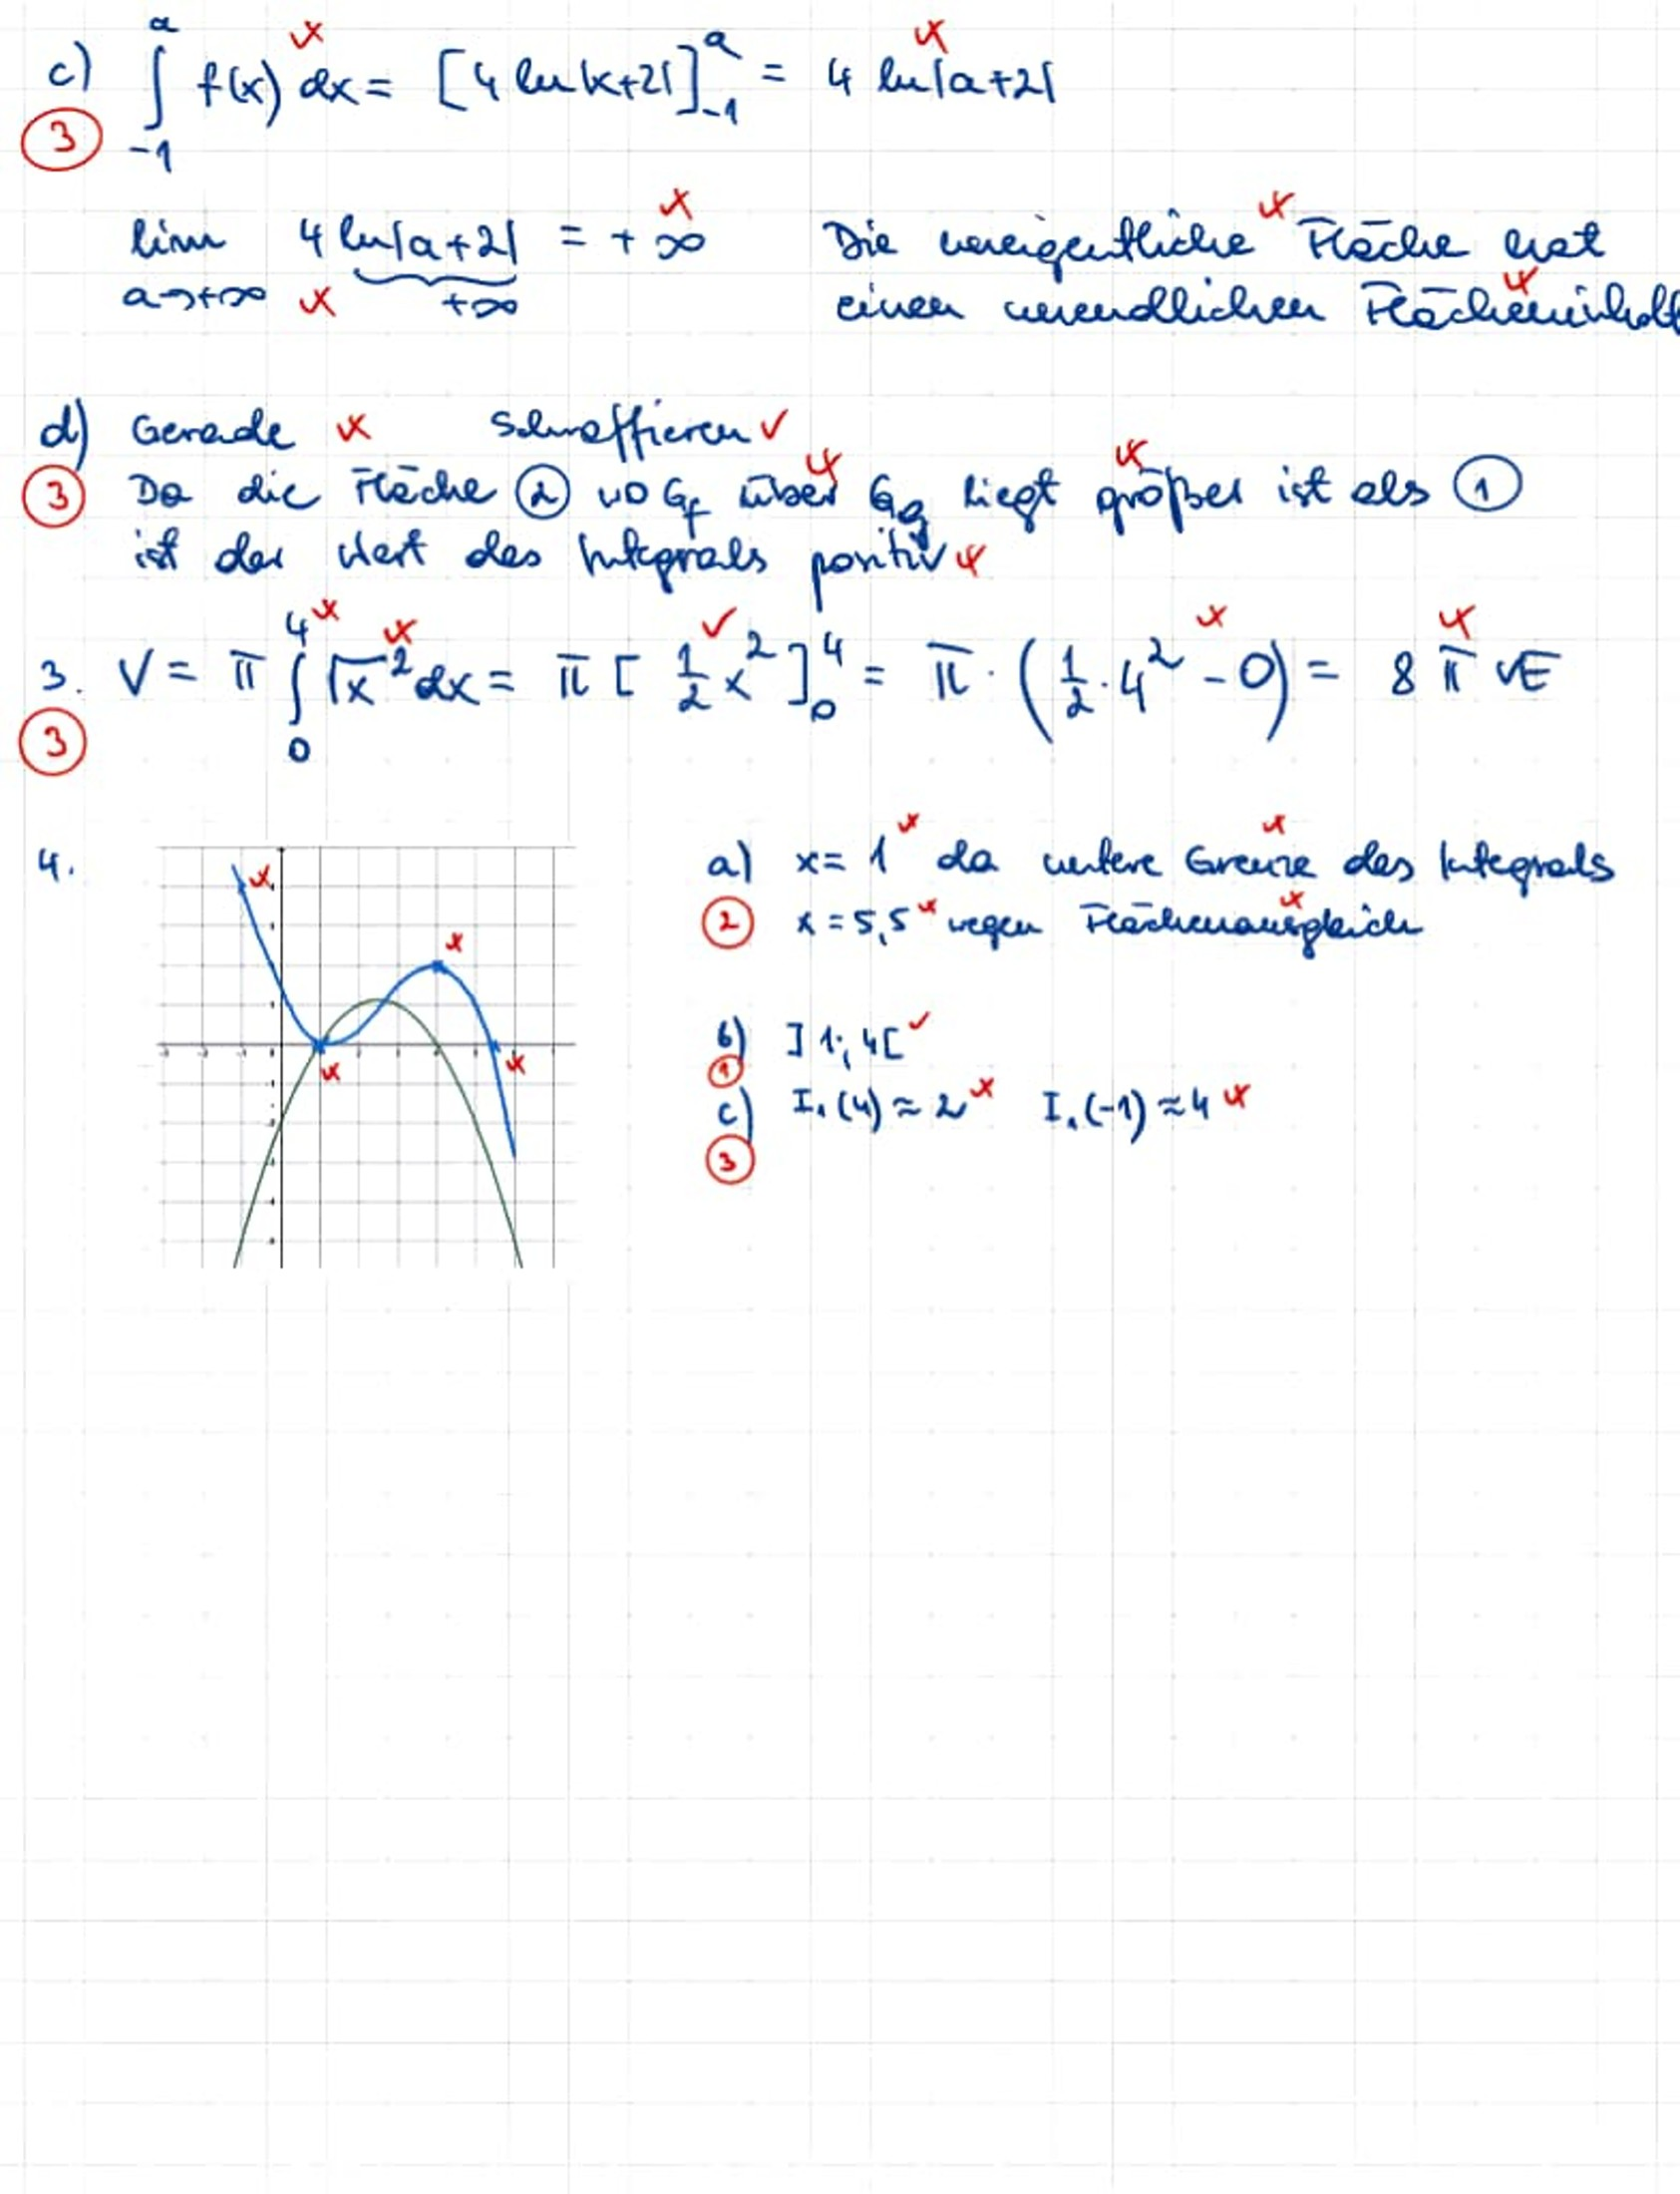
\includegraphics[width=1.2\linewidth]{Q12_SA_240103_10.jpg}
  \end{figure}

\newpage
  \begin{figure}[H]
    \vspace{0cm}
    \centering
    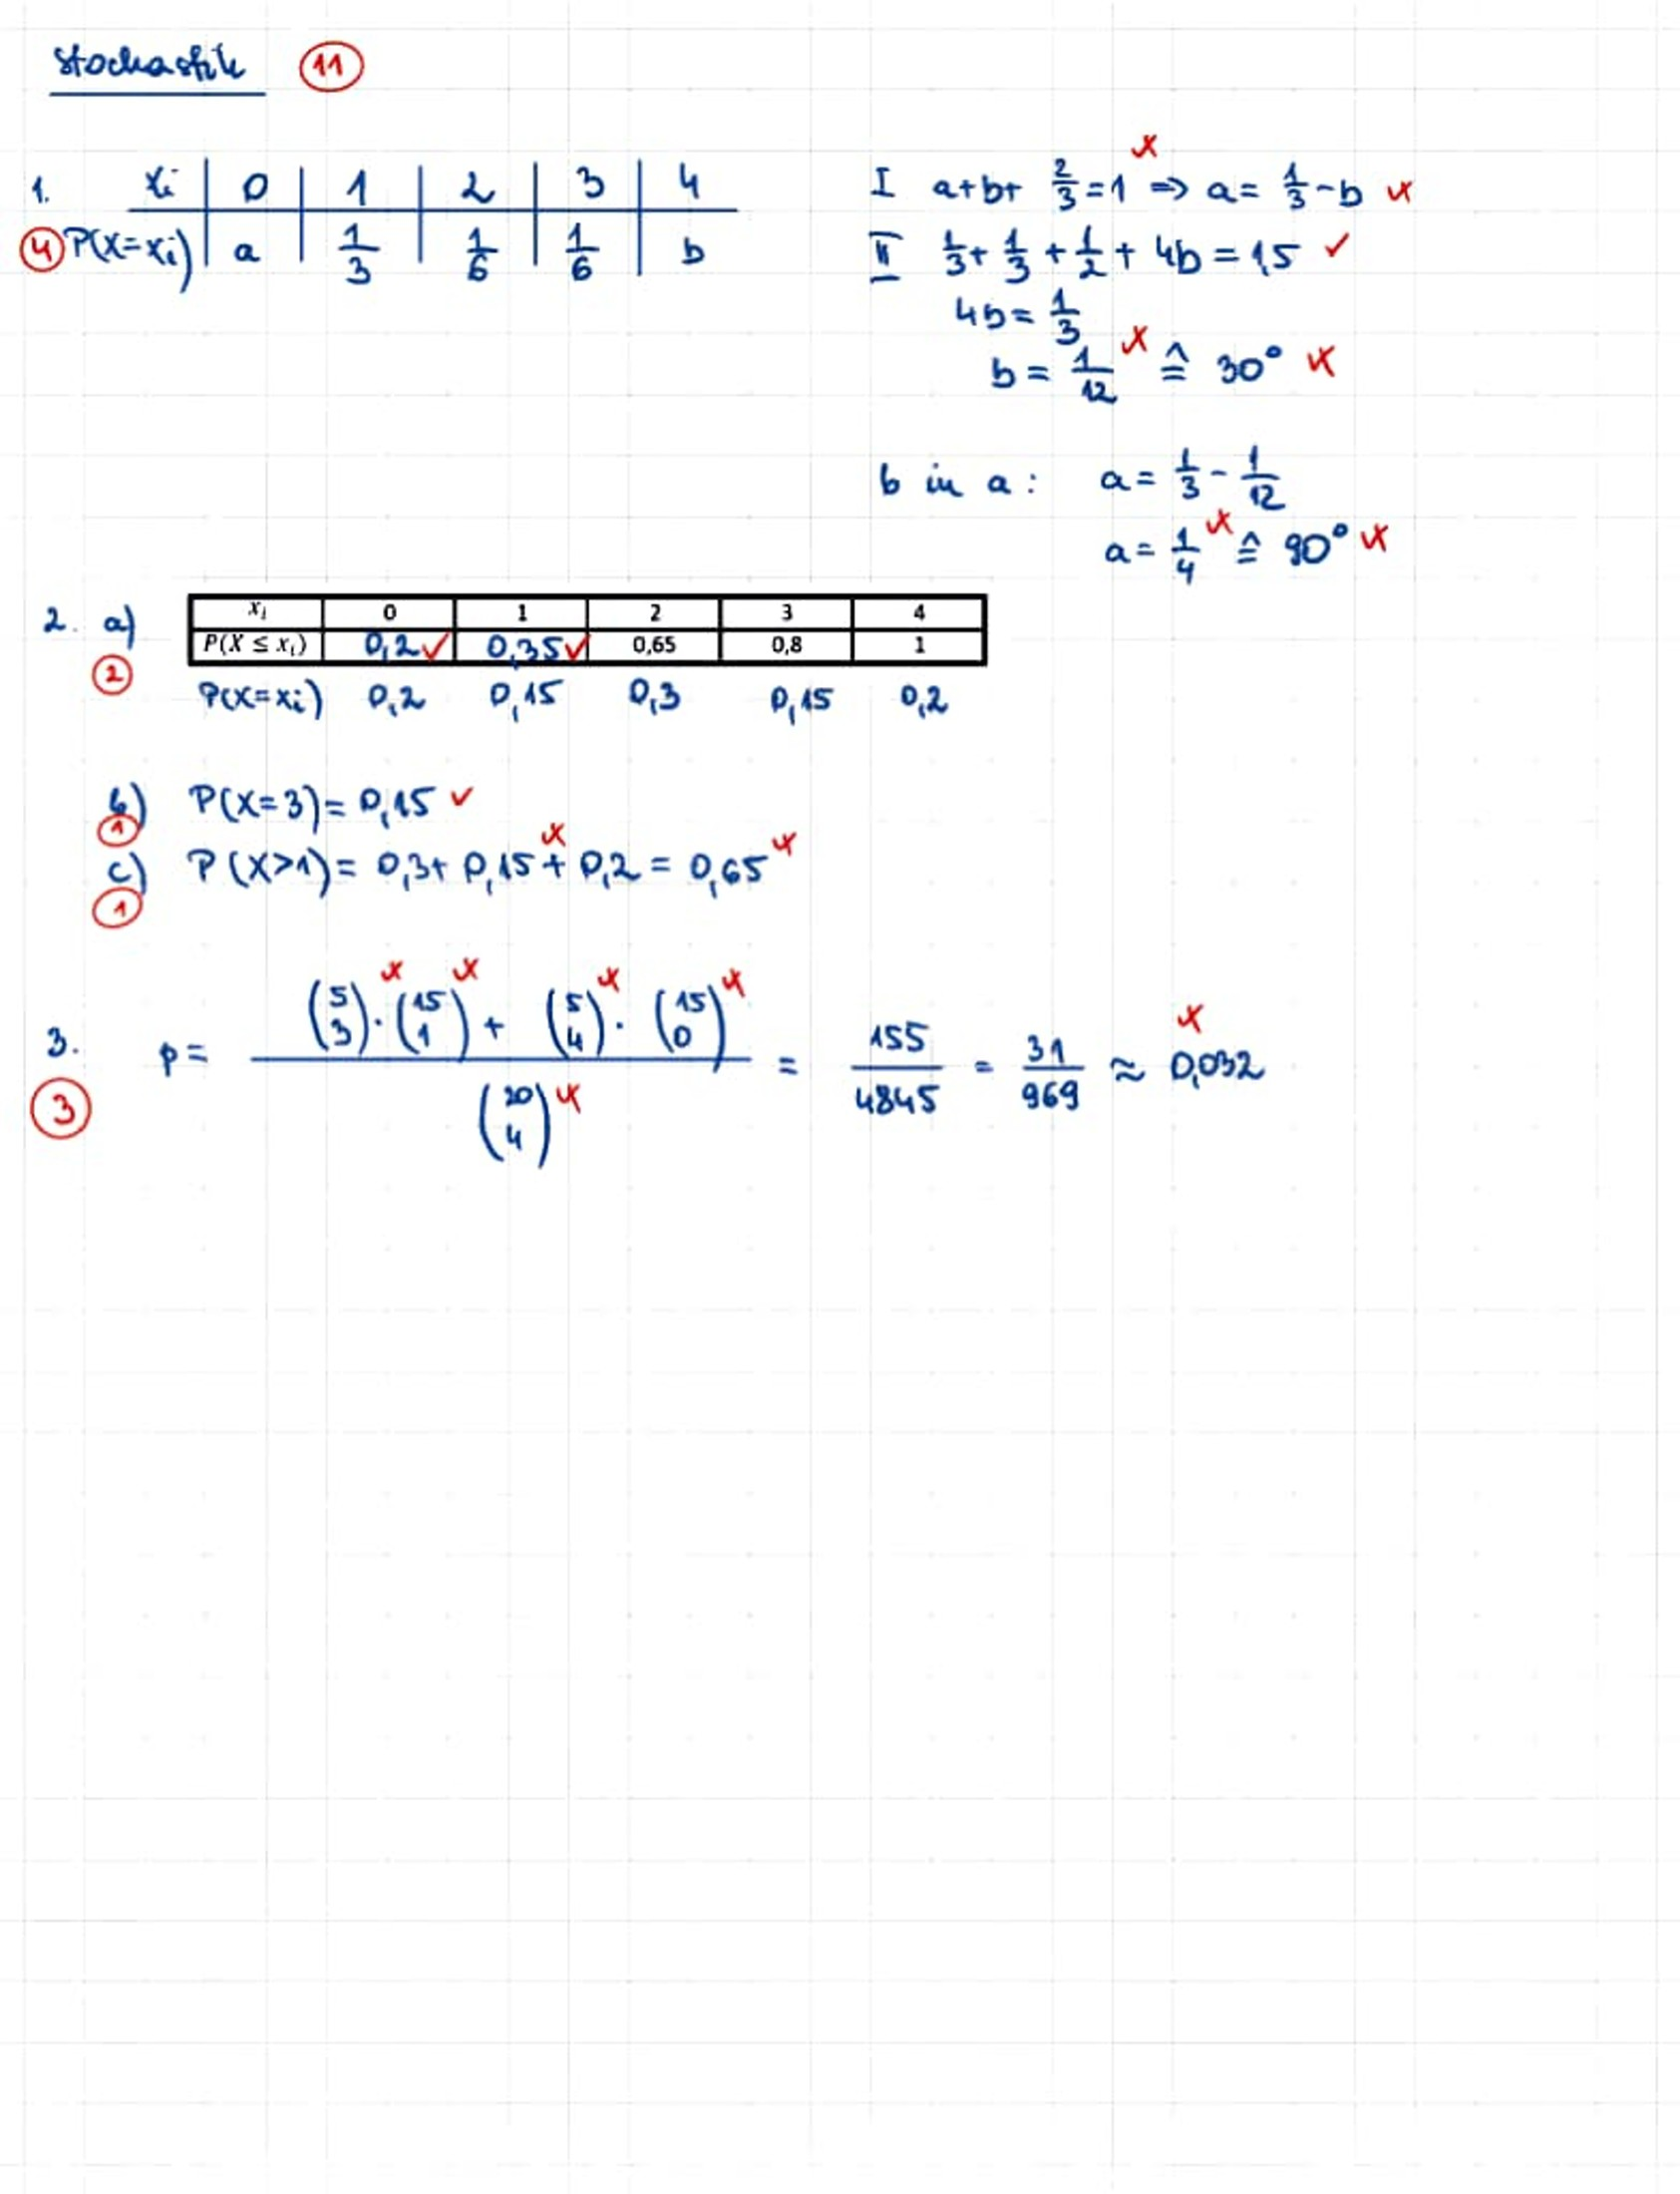
\includegraphics[width=1.2\linewidth]{Q12_SA_240103_11.jpg}
  \end{figure}

\end{document}
